\documentclass[conference]{IEEEtran}
\IEEEoverridecommandlockouts

\usepackage{cite}
\usepackage{amsmath,amssymb,amsfonts}
\usepackage{graphicx}
\usepackage{textcomp}
\usepackage{xcolor}
\usepackage{booktabs}
\usepackage{array}
\newcolumntype{L}[1]{>{\raggedright\arraybackslash}p{#1}}
\usepackage{multirow}
\usepackage{xurl}
\usepackage[hidelinks]{hyperref}

% Placeholder for text still to be written or numbers still to be confirmed.
% Search for \todo before submission: none may remain.
\newcommand{\todo}[1]{\textcolor{red}{\textbf{[TODO: #1]}}}
% Highlighted finding after each research question.
\newcommand{\finding}[2]{%
  \par\smallskip\noindent\fbox{\parbox{\dimexpr\columnwidth-2\fboxsep-2\fboxrule\relax}{%
  \textbf{Finding #1.} #2}}\par\smallskip}
\newcommand{\so}{\texttt{set-output}}
\newcommand{\art}{artifact actions}

\begin{document}

\title{Warn or Break? How Open-Source Projects Respond to\\
Platform-Enforced Deprecations in GitHub Actions}

\author{\IEEEauthorblockN{\todo{Given Name Surname}}
\IEEEauthorblockA{\textit{\todo{Faculty / department}} \\
\textit{\todo{University}}\\
\todo{City, Country} \\
\todo{email}}
}

\maketitle

\begin{abstract}
\todo{Abstract, written last (150--200 words): context, what we study, data, main findings with numbers, implication.}
\end{abstract}

\begin{IEEEkeywords}
GitHub Actions, deprecation, continuous integration, software ecosystems, mining software repositories
\end{IEEEkeywords}

\section{Introduction}\label{sec:intro}

\todo{Written after the results. Planned content:
(1) GitHub Actions is the dominant CI service; workflows depend on platform components that GitHub maintains and periodically deprecates.
(2) Platforms must choose how to end support: warn, break, or warn and then withdraw; little is known about how projects respond.
(3) We treat two GitHub deprecations with different endings as natural experiments.
(4) Data and approach in one sentence.
(5) Main findings (three bullets with numbers).
(6) Contributions and replication package.}

\section{Background}\label{sec:background}

\subsection{GitHub Actions}
GitHub Actions runs the continuous integration (CI) of a repository from YAML \emph{workflow} files stored in \texttt{.github/workflows}.
A workflow consists of jobs, and each job of steps that either run shell commands (\texttt{run:}) or call a reusable \emph{action} referenced by owner, name and version (\texttt{uses: actions/checkout@v4}).
Workflows therefore depend on two kinds of platform components that GitHub maintains: the official actions published under the \texttt{actions/} organization, and the \emph{workflow commands} through which a step talks to the runner, written as special lines to standard output.
When GitHub changes one of these components it deprecates the old one: it announces the change in its changelog, shows a warning in the log of every affected run, and names a date after which the old component stops working.
How that date is handled differs from one deprecation to the next.
We study two deprecations that ended in opposite ways (Table~\ref{tab:events}).

\subsection{Artifact actions v1--v3: an enforced cutoff}
The actions \texttt{actions/upload-artifact} and \texttt{actions/download-artifact} store files produced by a job (build outputs, test reports, logs) and pass them between jobs.
Version~4, released in December~2023, moved artifacts to a new storage backend.
On 16~April~2024 GitHub announced that versions~1--3 were deprecated~\cite{gh-artifact-deprecation}: v1 and v2 would stop working on 30~June~2024 and v3 on 30~January~2025.
Before the v3 cutoff GitHub ran three announced \emph{brownouts}, short windows in which v3 workflows failed on purpose, on 9, 16 and 23~January~2025 (1, 4 and 8 hours)~\cite{gh-artifact-brownouts}.
After the cutoff every run that uses a deprecated version fails.
Migrating is not always a version bump: v4 artifacts are immutable, so a workflow that uploaded several times to the same artifact name, for example from a build matrix, has to use unique names and merge them afterwards.

\subsection{\so{} and \texttt{save-state}: a withdrawn cutoff}
A step passes values to later steps with the workflow command \texttt{echo "::set-output name=<key>::<value>"}, and an action keeps state between its phases with \texttt{::save-state}.
Because the runner parsed these commands from anything printed to standard output, untrusted text written to a log, such as the title of a pull request, could inject outputs.
On 11~October~2022 GitHub deprecated both commands in favour of writing to the files named by \texttt{\$GITHUB\_OUTPUT} and \texttt{\$GITHUB\_STATE}, and announced that they would be disabled on 31~May~2023~\cite{gh-setoutput-deprecation}.
On 24~July~2023 GitHub postponed the removal indefinitely because its telemetry still showed significant use~\cite{gh-setoutput-deprecation}.
The commands still work today and only print a warning.

\begin{table}[t]
\caption{The two deprecation events}\label{tab:events}
\centering\footnotesize
\begin{tabular}{@{}L{0.17\columnwidth}L{0.37\columnwidth}L{0.36\columnwidth}@{}}
\toprule
 & \textbf{Artifact actions v1--v3} & \textbf{\so{}, \texttt{save-state}} \\
\midrule
Deprecated & action versions (\texttt{uses:}) & workflow commands (\texttt{run:}) \\
Notice ($T_{warn}$) & 2024-04-16 & 2022-10-11 \\
Brownouts & 2025-01-09, 16, 23 (v3) & none \\
Cutoff & 2024-06-30 (v1/v2), 2025-01-30 (v3) & announced for 2023-05-31 \\
Outcome & enforced: workflows fail & postponed on 2023-07-24 \\
Fix & \texttt{@v4}, sometimes unique names & write to \texttt{\$GITHUB\_OUTPUT} \\
\bottomrule
\end{tabular}
\end{table}

\section{Research Questions}\label{sec:rqs}

The two events share a warning period but end differently: one with an enforced cutoff that breaks CI, the other with a cutoff that was announced and then withdrawn.
We use this contrast to ask how projects respond.

\textbf{RQ1: When do projects migrate away from a deprecated component?}
We place each migration on the timeline of its deprecation: before anything broke, during the brownouts, after the cutoff, or never.
This tells whether warnings alone move projects, or only breakage does.

\textbf{RQ2: How does the way a deprecation ends affect the speed and extent of migration?}
We compare the time to migration under the enforced and the withdrawn cutoff, overall and within repositories exposed to both.

\textbf{RQ3: Which project characteristics are associated with timely migration?}
We relate migrating before any breakage to the size, activity and dependency tooling (Dependabot, Renovate) of a project.

\textbf{RQ4: Who performs the migrations?}
We classify the author of each migration as a dependency bot, a core maintainer or an external contributor.

\textbf{RQ5: How do projects migrate, and what problems do they meet?}
We code each migration by the kind of change, what triggered it, and the problems visible in the commits.

\section{Dataset Curation}\label{sec:data}

\subsection{Sampling}
We drew the repositories from SEART GitHub Search~\cite{dabic2021seart}, exported on 28~October~2026 with the filters in Table~\ref{tab:frame}.
Repositories created before 2022 existed through both events, and a commit after the last cutoff (February~2025) shows that a project was still maintained when a migration became unavoidable.
The thresholds on stars, contributors and commits restrict the frame to established, collaborative projects, the population for which questions about who migrates and how quickly are meaningful.
The export holds 22,608 repositories; we dropped the 393 archived ones, which can no longer change.
We shuffled the remaining 22,215 with a fixed seed and took the first 500, a simple random sample that later batches can extend.
One sampled repository no longer existed, and two sampled names turned out to be the same repository under its old and new name, which we counted once.
The sample therefore has 498 distinct repositories.

\begin{table}[t]
\caption{Sampling frame (SEART GitHub Search, 2026-10-28)}\label{tab:frame}
\centering\small
\begin{tabular}{@{}ll@{}}
\toprule
\textbf{Filter} & \textbf{Value} \\
\midrule
Created & before 2022-01-01 \\
Last commit & on or after 2025-02-01 \\
Stars / contributors / commits & $\geq$ 500 / $\geq$ 10 / $\geq$ 500 \\
Forks, archived & excluded \\
\midrule
Frame / sample & 22,215 / 498 repositories \\
\bottomrule
\end{tabular}
\end{table}

\subsection{Data collection}
We cloned every repository with its full commit history (without file contents, which git fetches on demand) on 28~October~2026, and analyzed the history of its default branch up to that day.
For each event and repository we scanned the files in \texttt{.github/workflows} at every relevant point of the first-parent history of the default branch, so that a change counts from the moment it reached the default branch, whether through a direct commit or a merge.

\textbf{Detection.}
For the artifact actions, a deprecated use is a \texttt{uses:} reference to \texttt{actions/upload-artifact} or \texttt{actions/download-artifact} at major version~1, 2 or~3, written as a major tag (\texttt{@v3}), a minor or patch tag (\texttt{@v3.1.3}), or a commit hash of one of those releases (we collected the hashes of all official v1--v3 tags).
Actions of other owners with similar names, such as \texttt{dawidd6/action-download-artifact}, do not count.
For the workflow commands, a deprecated use is the string \texttt{::set-output} or \texttt{::save-state}.
Commented-out lines are ignored for both.

\textbf{Exposure and migration.}
A repository is \emph{exposed} to an event if its default branch contained at least one deprecated use on the day of the deprecation notice ($T_{warn}$).
For an exposed repository, the \emph{migration} is the earliest default-branch commit after $T_{warn}$ after which no deprecated use remains; a repository with uses left on the collection day did not migrate.
For the artifact actions we treat v1/v2 and v3 separately, because their cutoffs differ: a migration counts as after the cutoff if any version group that the repository used at $T_{warn}$ disappeared only after that group's cutoff.

Of the 498 repositories, 124 were exposed to at least one event: 90 to the artifact deprecation, 57 to the \so{} deprecation and 23 to both, giving 147 (repository, event) pairs.

\subsection{Validation}
We developed the detection rules on a separate, hand-picked set of 90 popular repositories, checking every detected case against its diff and commit message.
This revealed the problems the final rules address: commented-out lines, look-alike third-party actions, migrations that reach the default branch only through a merge, and repositories that mixed v2 and v3.
\todo{Independent validation on the sample (manual\_validation.xlsx): A -- of 30 randomly sampled migrations, X removed the deprecated use as detected (precision); C -- of the 14 non-migrated pairs, Y still contained an active deprecated use in the collected snapshot; B -- agreement of the author classification with GitHub's author-association badge on 30 migrations.}

\section{Data Analysis}\label{sec:analysis}

\textbf{Time and censoring.}
For every pair we measure time in days from the event's deprecation notice.
Pairs that never migrated are right-censored at the repository's last commit or at data collection, whichever is earlier: a project that stopped committing had no further chance to migrate.

\textbf{RQ1.}
We assign each migration to a phase of its event's timeline.
For the artifact actions the phases are \emph{before any breakage} (before the first brownout for v3, before the cutoff for v1/v2), \emph{during the brownouts} (9--29~January~2025), and \emph{after the cutoff}.
For \so{} they are \emph{before the announced cutoff} (31~May~2023), \emph{between the announced cutoff and its postponement} (24~July~2023), and \emph{after the postponement}.
We also plot migrations per calendar week against the key dates.

\textbf{RQ2.}
We estimate the share of exposed repositories still using the deprecated component over time with the Kaplan--Meier estimator~\cite{kaplan1958} and compare the two events with the log-rank test~\cite{mantel1966}.
Because the events differ in period and in the projects they reach, we also compare, within the repositories that migrated away from both, the time each migration took (Wilcoxon signed-rank test).
As a sensitivity check we repeat the comparison with all non-migrants censored at the collection date.

\textbf{RQ3.}
We call a migration \emph{timely} if it happened before anything broke (before any breakage for the artifact actions, before the announced cutoff for \so{}).
For each pair we measured, on the default branch at $T_{warn}$: whether Dependabot was configured to update GitHub Actions and whether a Renovate configuration existed; the commits and distinct authors in the preceding six months; the number of workflow files; and the number of deprecated uses.
Stars, contributors and age come from the SEART export.
We compare timely and other pairs with the Mann--Whitney U test and Fisher's exact test, and fit, per event, a Cox proportional-hazards model~\cite{cox1972} of the time to migration with four covariates (stars, prior commits and deprecated uses on a log scale, and whether Dependabot or Renovate was configured), about one covariate per ten migrations.
We correct each family of p-values with Holm's method~\cite{holm1979} and check the proportional-hazards assumption by correlating each covariate's Schoenfeld residuals with event time~\cite{grambsch1994}.

\textbf{RQ4.}
For each migration we identify the commit that removed the last deprecated use; when the migration reached the default branch through a merge, this is the commit inside the merge, not the merge itself.
Its author is a \emph{bot} if the name identifies a dependency or automation bot (Dependabot, Renovate, GitHub Actions).
A human author is a \emph{core maintainer} if, in the year before the migration, they authored at least 10 commits or at least 10\% of the default-branch commits (and at least 3), or authored a merge commit, or if the change was merged from a branch of the repository itself, which requires write access.
Other authors are \emph{external contributors}.
We also record whether a bot initiated a change that a human finished.

\textbf{RQ5.}
For every pair we collected the commit messages of the change and of the merge that brought it in, the workflow diff, follow-up commits to the same workflows within 30 days, and, for pairs that did not migrate, the remaining uses.
We coded each pair along three dimensions (Table~\ref{tab:codebook}): the \emph{change type}, the \emph{trigger} stated in the messages, and the \emph{problems} visible in the material.
The codes were derived inductively on the hand-picked set and then applied to all 147 pairs.
\todo{Reliability of the RQ5 coding: who coded, and agreement (Cohen's kappa~\cite{cohen1960}) on the independently coded subset D of manual\_validation.xlsx.}

\begin{table}[t]
\caption{RQ5 codebook (abridged)}\label{tab:codebook}
\centering\footnotesize
\begin{tabular}{@{}lL{0.64\columnwidth}@{}}
\toprule
\multicolumn{2}{@{}l}{\textbf{Change type} (one per pair)} \\
\texttt{bump} & one-to-one replacement (new version, \texttt{\$GITHUB\_OUTPUT}) \\
\texttt{adapt} & replacement plus changes the new behaviour required \\
\texttt{remove} & step or workflow deleted instead of replaced \\
\texttt{replace} & a different mechanism takes over \\
\midrule
\multicolumn{2}{@{}l}{\textbf{Trigger} (first that applies)} \\
\texttt{bot} & authored or initiated by a dependency bot \\
\texttt{breakage} & message reports a failing build \\
\texttt{deprecation} & message names the deprecation or its warning \\
\texttt{targeted} & change aimed at the component, no reason given \\
\texttt{routine} & general update of actions or dependencies \\
\texttt{incidental} & part of unrelated work \\
\midrule
\multicolumn{2}{@{}l}{\textbf{Problems} (one or more)} \\
\texttt{incompatibility} & new version forced extra changes or a repair \\
\texttt{environment} & runner or container could not run the new version \\
\texttt{regression} & migration introduced an error fixed later \\
\texttt{multiline} & multi-line output values broke \\
\texttt{deferral} & explicit decision to keep the old version \\
\bottomrule
\end{tabular}
\end{table}

\section{Results}\label{sec:results}

\subsection{RQ1: When do projects migrate?}\label{sec:rq1}

Table~\ref{tab:phases} places every exposed repository on the timeline of its deprecation.
For the artifact actions, only 30 of 90 repositories (33\%) migrated while nothing had broken yet, although the warning period lasted more than nine months for v3.
Four more migrated during the brownouts in January~2025, and 51 (57\%) migrated only after their workflows had started to fail.
Five never migrated.
For \so{}, 25 of 57 repositories (44\%) migrated before the announced cutoff, one in the eight weeks between the announced date and its postponement, 22 (39\%) after the postponement, and nine never did.

\begin{table}[t]
\caption{RQ1: Phase of the migration on the timeline of each deprecation}\label{tab:phases}
\centering\footnotesize
\begin{tabular}{@{}L{0.42\columnwidth}rr@{\hspace{10pt}}L{0.24\columnwidth}@{}}
\toprule
\textbf{Phase} & \textbf{Repos} & \textbf{\%} & \\
\midrule
\multicolumn{4}{@{}l}{\textit{Artifact actions v1--v3 (n = 90), enforced cutoff}} \\
Before any breakage & 30 & 33.3 & \\
During the v3 brownouts & 4 & 4.4 & \\
After the cutoff (CI broken) & 51 & 56.7 & \\
Not migrated & 5 & 5.6 & \\
\midrule
\multicolumn{4}{@{}l}{\textit{\so{} (n = 57), withdrawn cutoff}} \\
Before the announced cutoff & 25 & 43.9 & \\
Between cutoff date and postponement & 1 & 1.8 & \\
After the postponement & 22 & 38.6 & \\
Not migrated & 9 & 15.8 & \\
\bottomrule
\end{tabular}
\end{table}

Fig.~\ref{fig:weekly} shows when the migrations happened.
Artifact migrations trickle in after the notice and then pile up twice: in September~2024, when v1/v2 workflows started to fail, and around the v3 brownouts and cutoff, each time followed by a tail of repositories that repaired their CI weeks or months later.
Neither announced date left a mark.
Of the 35 repositories that used v1 or v2 at the notice and later dropped them, three did so before the announced cutoff of 30~June~2024 and four in the ten weeks during which the old versions still worked after it; eleven followed within two weeks of the first failure reports, and the remaining 17 later.
Around the first announced v3 date, 30~November~2024, the v3 migrations show no increase either.
The \so{} migrations follow the opposite shape: a burst in the first weeks after the notice, steady migration until the announced cutoff, and only a thin tail after GitHub postponed it.

\begin{figure*}[t]
\centering
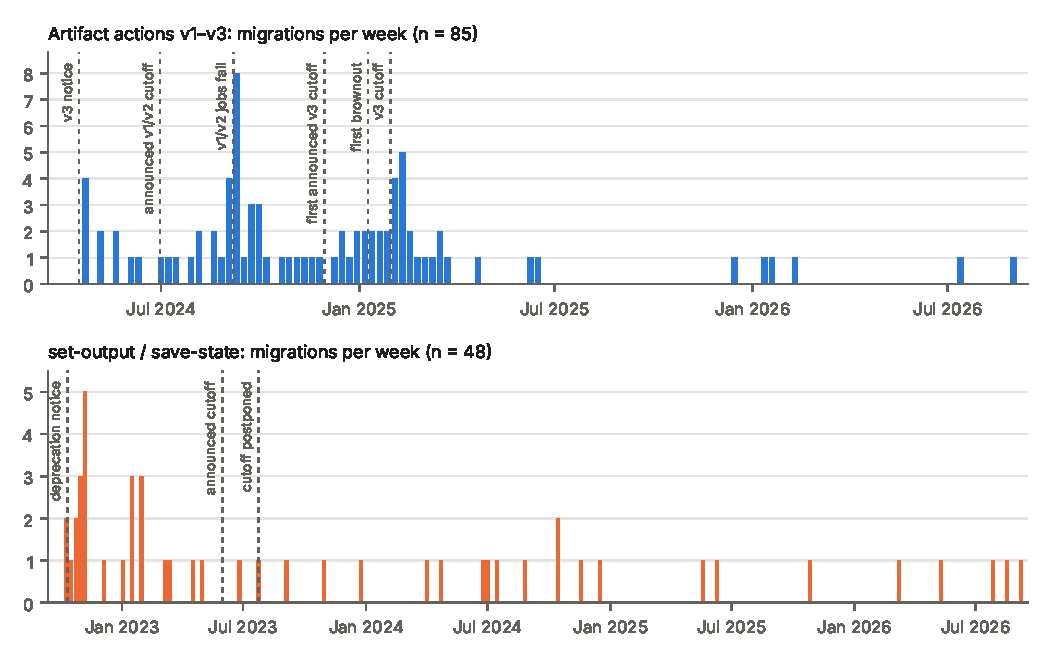
\includegraphics[width=0.9\textwidth]{figures/sample_weekly.pdf}
\caption{Migrations per calendar week. Dashed lines mark the key dates of each deprecation.}\label{fig:weekly}
\end{figure*}

\finding{1}{Warnings alone moved a minority of projects. For the enforced deprecation, 57\% of the exposed projects migrated only after their CI had broken, and migrations followed the days on which workflows actually failed, not the announced dates. For the withdrawn deprecation, migration happened mostly before the announced cutoff and nearly stopped after it was postponed.}

\subsection{RQ2: Does the way a deprecation ends matter?}\label{sec:rq2}

Fig.~\ref{fig:km} and Table~\ref{tab:survival} compare how long repositories kept using the deprecated component.
The \so{} curve falls faster at first: 19\% of the exposed repositories had migrated after 30~days, against 7\% for the artifact actions.
The picture reverses once the first artifact workflows fail: the artifact curve drops steeply in September~2024 and again around the v3 brownouts and cutoff, while the \so{} curve flattens after the postponement.
One year after the notice, 85\% of the artifact-exposed repositories had migrated, but only 49\% of the \so{}-exposed ones; the median time to migration was 224 and 384 days.
The difference is significant (log-rank $\chi^2 = 12.8$, $p < 0.001$) and remains so when non-migrants are censored at the collection date instead of their last commit ($\chi^2 = 11.3$, $p < 0.001$).

\begin{figure*}[t]
\centering
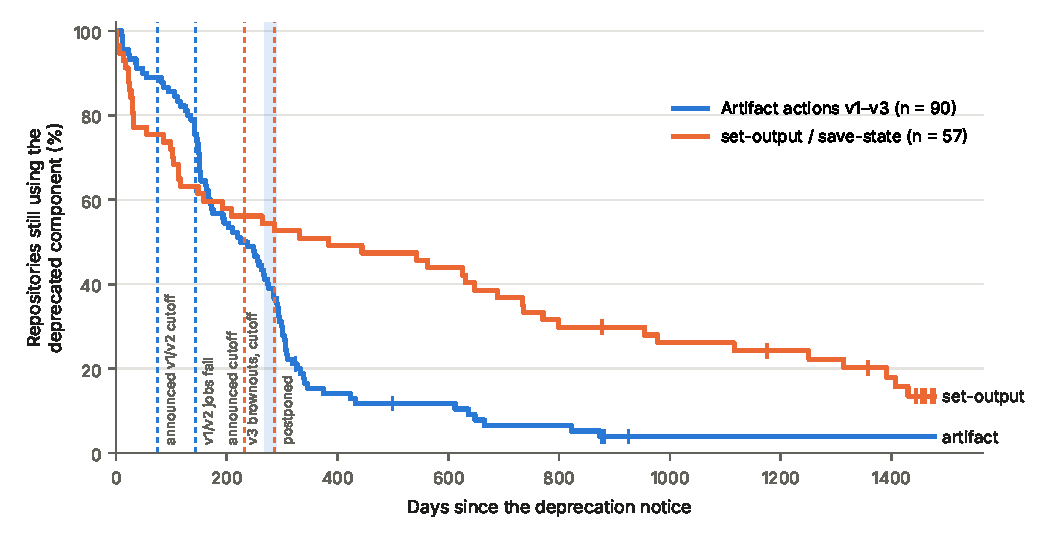
\includegraphics[width=0.9\textwidth]{figures/sample_km.pdf}
\caption{Share of exposed repositories still using the deprecated component, by days since the deprecation notice (Kaplan--Meier estimate; ticks mark censored repositories).}\label{fig:km}
\end{figure*}

\begin{table}[t]
\caption{RQ2: Time to migration (Kaplan--Meier)}\label{tab:survival}
\centering\footnotesize
\begin{tabular}{@{}lrrrrrr@{}}
\toprule
 & & \multicolumn{5}{c}{\textbf{Migrated after (\%)}} \\
\cmidrule(l){3-7}
\textbf{Event} & \textbf{Median} & \textbf{30\,d} & \textbf{90\,d} & \textbf{180\,d} & \textbf{1\,y} & \textbf{2\,y} \\
\midrule
Artifact actions & 224\,d & 6.7 & 13.3 & 43.3 & 84.8 & 93.5 \\
\so{} & 384\,d & 19.3 & 26.3 & 40.4 & 49.1 & 63.2 \\
\bottomrule
\end{tabular}
\end{table}

The two events differ in more than their ending, so we also compare the 18 repositories that migrated away from both.
Twelve of them took less time for the artifact actions than for \so{}, with a median difference of 296~days (Wilcoxon signed-rank, $p = 0.021$).
The same projects, then, reacted faster to the deprecation that was enforced.

\finding{2}{An enforced cutoff led to faster and more complete migration than a cutoff that was announced and then withdrawn (85\% vs.\ 49\% migrated within a year), also within the same projects. The withdrawn cutoff started faster but stalled once the threat disappeared.}

\subsection{RQ3: Which projects migrate in time?}\label{sec:rq3}

Projects that migrated before anything broke looked much like the others.
None of the nine characteristics we compared differed significantly after Holm's correction (Table~\ref{tab:cox}).
Two associations are suggestive.
For the artifact actions, projects that migrated in time more often had Dependabot or Renovate configured (17\% vs.\ 3\%, $p = 0.039$ uncorrected) and had been somewhat more active in the six months before the notice (median 96 vs.\ 62 commits, $p = 0.060$); in the Cox model more prior activity went with faster migration (HR 1.14 per e-fold increase).
For \so{}, projects with Dependabot or Renovate configured migrated faster (HR 2.39), although not a single \so{} migration was made by a bot (RQ4): the tools seem to mark projects that look after their CI rather than doing the work.
For both events the effect of these tools also changes over time (Schoenfeld residuals correlate with time, $\rho \approx 0.5$), so the hazard ratio is only an average.
Stars, contributors, age, the number of workflow files and the number of deprecated uses showed no association.

\begin{table}[t]
\caption{RQ3: Cox models of the time to migration}\label{tab:cox}
\centering\footnotesize
\begin{tabular}{@{}lrlrr@{}}
\toprule
\textbf{Covariate} & \textbf{HR} & \textbf{95\% CI} & \textbf{p} & \textbf{p (Holm)} \\
\midrule
\multicolumn{5}{@{}l}{\textit{Artifact actions (n = 90, 85 migrations)}} \\
Stars ($\log_{10}$) & 0.68 & 0.44--1.05 & 0.082 & 0.49 \\
Commits, 6 months before ($\log$) & 1.14 & 1.02--1.28 & 0.026 & 0.18 \\
Deprecated uses ($\log$) & 0.91 & 0.64--1.29 & 0.603 & 1.00 \\
Dependabot or Renovate & 1.87 & 0.83--4.20 & 0.130 & 0.65 \\
\midrule
\multicolumn{5}{@{}l}{\textit{\so{} (n = 57, 48 migrations)}} \\
Stars ($\log_{10}$) & 1.58 & 0.84--2.98 & 0.155 & 0.65 \\
Commits, 6 months before ($\log$) & 1.04 & 0.84--1.29 & 0.716 & 1.00 \\
Deprecated uses ($\log$) & 1.28 & 0.78--2.09 & 0.330 & 0.99 \\
Dependabot or Renovate & 2.39 & 1.21--4.72 & 0.012 & 0.10 \\
\bottomrule
\end{tabular}
\end{table}

One observation qualifies these results.
Only 5 of the 90 artifact-exposed repositories had Dependabot configured for GitHub Actions on the day of the notice.
Version~4 had been available for four months by then, so most projects with Dependabot had already been moved to it automatically and were never exposed.
Dependency bots thus act \emph{before} a deprecation, by keeping projects off outdated versions, which our design, conditioned on exposure, cannot capture.

\finding{3}{No project characteristic reliably predicts timely migration. Prior activity and the use of dependency bots point in the expected direction but do not survive correction for multiple testing. Bots mainly keep projects from being exposed in the first place.}

\subsection{RQ4: Who migrates?}\label{sec:rq4}

Table~\ref{tab:authors} shows who authored the change that removed the last deprecated use.
Core maintainers did most of the work: 74\% of the artifact migrations and 94\% of the \so{} migrations.
Bots authored only 4 artifact migrations, all of them version bumps made before anything broke, and no \so{} migration, which a version bump cannot fix.
External contributors authored 21\% of the artifact migrations.
Their share was higher before anything broke (30\%) than after the cutoff (16\%): when CI failed, maintainers fixed it themselves.

\begin{table}[t]
\caption{RQ4: Author of the migration}\label{tab:authors}
\centering\footnotesize
\begin{tabular}{@{}lrrrr@{}}
\toprule
\textbf{Event / phase} & \textbf{n} & \textbf{Bot} & \textbf{Core} & \textbf{External} \\
\midrule
\textit{Artifact actions} & 85 & 4 (5\%) & 63 (74\%) & 18 (21\%) \\
\quad before any breakage & 30 & 4 & 17 & 9 \\
\quad during the brownouts & 4 & 0 & 3 & 1 \\
\quad after the cutoff & 51 & 0 & 43 & 8 \\
\midrule
\textit{\so{}} & 48 & 0 (0\%) & 45 (94\%) & 3 (6\%) \\
\quad before the announced cutoff & 25 & 0 & 25 & 0 \\
\quad after the cutoff date & 23 & 0 & 20 & 3 \\
\bottomrule
\end{tabular}
\end{table}

\finding{4}{Migrations are maintenance work done by core maintainers. Bots contributed almost nothing once a project was exposed, and external contributors helped mostly before anything broke.}

\subsection{RQ5: How do projects migrate, and what goes wrong?}\label{sec:rq5}

Table~\ref{tab:rq5} summarizes the coding.
Most migrations were one-to-one replacements: 73\% of the artifact pairs and 60\% of the \so{} pairs.
For the artifact actions, 13\% needed further changes that v4 forced, and \so{} was more often removed or replaced by another mechanism (25\%), typically when a workflow was rewritten.

\begin{table}[t]
\caption{RQ5: Change type, trigger and problems}\label{tab:rq5}
\centering\footnotesize
\begin{tabular}{@{}lrr@{}}
\toprule
 & \textbf{Artifact} & \textbf{\so{}} \\
\midrule
\multicolumn{3}{@{}l}{\textit{Change type (all exposed pairs)}} \\
\texttt{bump} & 66 (73\%) & 34 (60\%) \\
\texttt{adapt} & 12 (13\%) & 0 \\
\texttt{remove} & 4 (4\%) & 5 (9\%) \\
\texttt{replace} & 3 (3\%) & 9 (16\%) \\
not migrated & 5 (6\%) & 9 (16\%) \\
\midrule
\multicolumn{3}{@{}l}{\textit{Trigger (migrations)}} \\
\texttt{bot} & 4 (5\%) & 0 \\
\texttt{breakage} & 13 (15\%) & 0 \\
\texttt{deprecation} & 14 (16\%) & 20 (42\%) \\
\texttt{targeted} & 22 (26\%) & 2 (4\%) \\
\texttt{routine} & 17 (20\%) & 6 (12\%) \\
\texttt{incidental} & 15 (18\%) & 20 (42\%) \\
\midrule
\multicolumn{3}{@{}l}{\textit{Problems (all exposed pairs)}} \\
\texttt{incompatibility} & 12 (13\%) & 0 \\
\texttt{environment} & 3 (3\%) & 0 \\
\texttt{regression} & 0 & 3 (5\%) \\
\texttt{multiline} & 0 & 3 (5\%) \\
\texttt{deferral} & 3 (3\%) & 0 \\
any problem & 16 (18\%) & 6 (11\%) \\
\bottomrule
\end{tabular}
\end{table}

\textbf{Triggers.}
The messages rarely say why a change was made.
For \so{}, 42\% of the migrations name the deprecation or its warning, and another 42\% happened as part of unrelated work.
For the artifact actions only 16\% name the deprecation; 15\% report a failing build, and all of those came during the brownouts (three of the four brownout migrations) or after the cutoff.
Several of these messages quote the error that GitHub printed, for example \texttt{microsoft/vcpkg-tool}, which migrated on 17~January~2025, the day after the second brownout.

\textbf{Problems.}
Problems were visible in 18\% of the artifact pairs and 11\% of the \so{} pairs.
For the artifact actions they were mostly incompatibilities of v4: workflows that uploaded to the same artifact name from every job of a build matrix had to give each job its own name and merge the artifacts afterwards (e.g., \texttt{mhammond/pywin32}, \texttt{qiskit/qiskit-aer}), and v4 stopped uploading hidden files by default (\texttt{flxzt/rnote}).
In three projects the runner environment was the obstacle: build containers with an old C library could not run the Node.js~20 that the new actions require, so projects moved the build out of the container or dropped the old platform (\texttt{academysoftwarefoundation/openfx}).
Three projects deliberately kept the old version for a while.
For \so{} the problems came from the new syntax itself: values written with a wrong key or broken quoting (\texttt{ardupilot/ardupilot}, \texttt{lightspark/lightspark}), and multi-line values that the new file format accepts only with a delimiter (\texttt{lucide-icons/lucide}).

\finding{5}{Most migrations were simple replacements, and most messages give no reason for them. When problems occurred, they came from behaviour changes of the new version (artifact actions) or from the new syntax (\so{}), and they explain part of the delay: a migration that needs workflow changes is not a one-line bump.}

\section{Discussion}\label{sec:discussion}

\subsection{Implications}
\todo{For platform maintainers: warnings in logs move few projects, breakage (including brownouts) moves most; a withdrawn cutoff stalls migration. For project maintainers and tool builders: dependency bots matter before a deprecation, not during it.}

\subsection{Threats to Validity}\label{sec:threats}
\todo{Write out each item.
\textbf{Construct}: exposure and migration are measured on the first-parent history of today's default branch (a later default-branch switch can delay the measured date); a fix on another branch counts only when merged; \so{} is detected only in workflow files, not inside third-party actions; brownouts lasted hours, so a migration on a brownout day may precede the failure; author roles are inferred from git history, not from GitHub's author association.
\textbf{Internal}: the two events differ in period, component and fix effort, not only in their ending; the within-repository comparison controls for the project but not for the period; non-migrants are censored.
\textbf{External}: established, collaborative projects only (SEART thresholds); two events of one platform.
\textbf{Reliability}: RQ5 codes are qualitative; detection validated manually; scripts and data are public and every result table is reproduced from them.}

\section{Related Work}\label{sec:related}

\todo{Three strands, each closing with how this study differs.
(1) Use and evolution of GitHub Actions: Kinsman et al.~\cite{kinsman2021}; Decan et al. on outdated workflows~\cite{decan2023}; studies of workflow evolution and maintenance (to collect).
(2) API deprecation and how developers react to it: Robbes et al. (Smalltalk), Hora et al., Sawant et al. (Java) (to collect).
(3) Dependency updates and bots: Dependabot and Renovate studies (to collect).
Gap: prior work treats deprecation-driven changes as a side finding or studies library APIs; none compares how the ending of a platform deprecation (enforced or withdrawn) shapes migration.}

\section{Conclusion}\label{sec:conclusion}

\todo{Summary of findings in three to four sentences and future work (more events, e.g. Node.js runtime transitions and runner image retirements; other CI platforms).}

\section*{Data Availability}
The scripts, the sample, all intermediate data and the result tables are available at \url{https://github.com/Mjavorr/ESS---research}. \todo{Archive a tagged release (e.g. on Zenodo) and cite its DOI.}


\bibliographystyle{IEEEtran}
\bibliography{references}

\end{document}
